\chapter{Introdução}\label{cap:introducao}

O uso de tecnologias de comunicação via satélite tem se mostrado fundamental para aplicações de \gls{IOT} em cenários remotos, especialmente no monitoramento ambiental, oceânico e meteorológico, através de plataformas equipadas com sensores, as chamadas \gls{PCD}, que são capazes de transmitir pequenas quantidades de dados periodicamente para satélites de órbita baixa \cite{Centenaro-2021, fraire_direct--satellite_2019}.

Dentre os sistemas internacionais voltados para esse tipo de aplicação, destaca-se o \gls{ARGOS} \footnote{https://www.argos-system.org/}, criado em 1978 por meio de uma cooperação entre o \gls{CNES}, \gls{NOAA} e \gls{NASA}. Desde seu desenvolvimento, o sistema \gls{ARGOS} tem passado por constantes evoluções, trazendo novos padrões de transmissão e modulação como os formatos \gls{PTT-A2}, \gls{PTT-A3} e \gls{PTT-ZE}, para aprimorar a eficiência espectral e a confiabilidade do enlace com o satélite. 

No Brasil, o \gls{SBCDA} \footnote{https://www.gov.br/aeb/pt-br/acoes-e-programas/aplicacoes-espaciais/dados-ambientais}, desenvolvido e operado pelo \gls{INPE}, emprega a tecnologia \gls{ARGOS}. O \gls{SBCDA} utiliza satélites em órbita baixa, como os \gls{SCD-1}, \gls{SCD-2} e os satélites da série \gls{CBERS}, para coletar dados transmitidos por \gls{PCD} instaladas em todo o território nacional \cite{rodrigues_demodulador_2018, duarte_multiuser_2021}. 

De acordo com dados do \gls{SINDA} \footnote{http://sinda.crn.inpe.br/PCD/}, atualmente é possível realizar a inspeção dos dados de 1030 pontos ativos de coleta distribuídos pelo país, cuja distribuição geográfica é apresentada na \autoref{fig:pcd_nacional} \cite{silva_um_2022}. 

\newpage
\begin{figure}[ht]
	\centering
	\caption{Mapa das PCDs distribuídas pelo território nacional}\label{fig:pcd_nacional}
	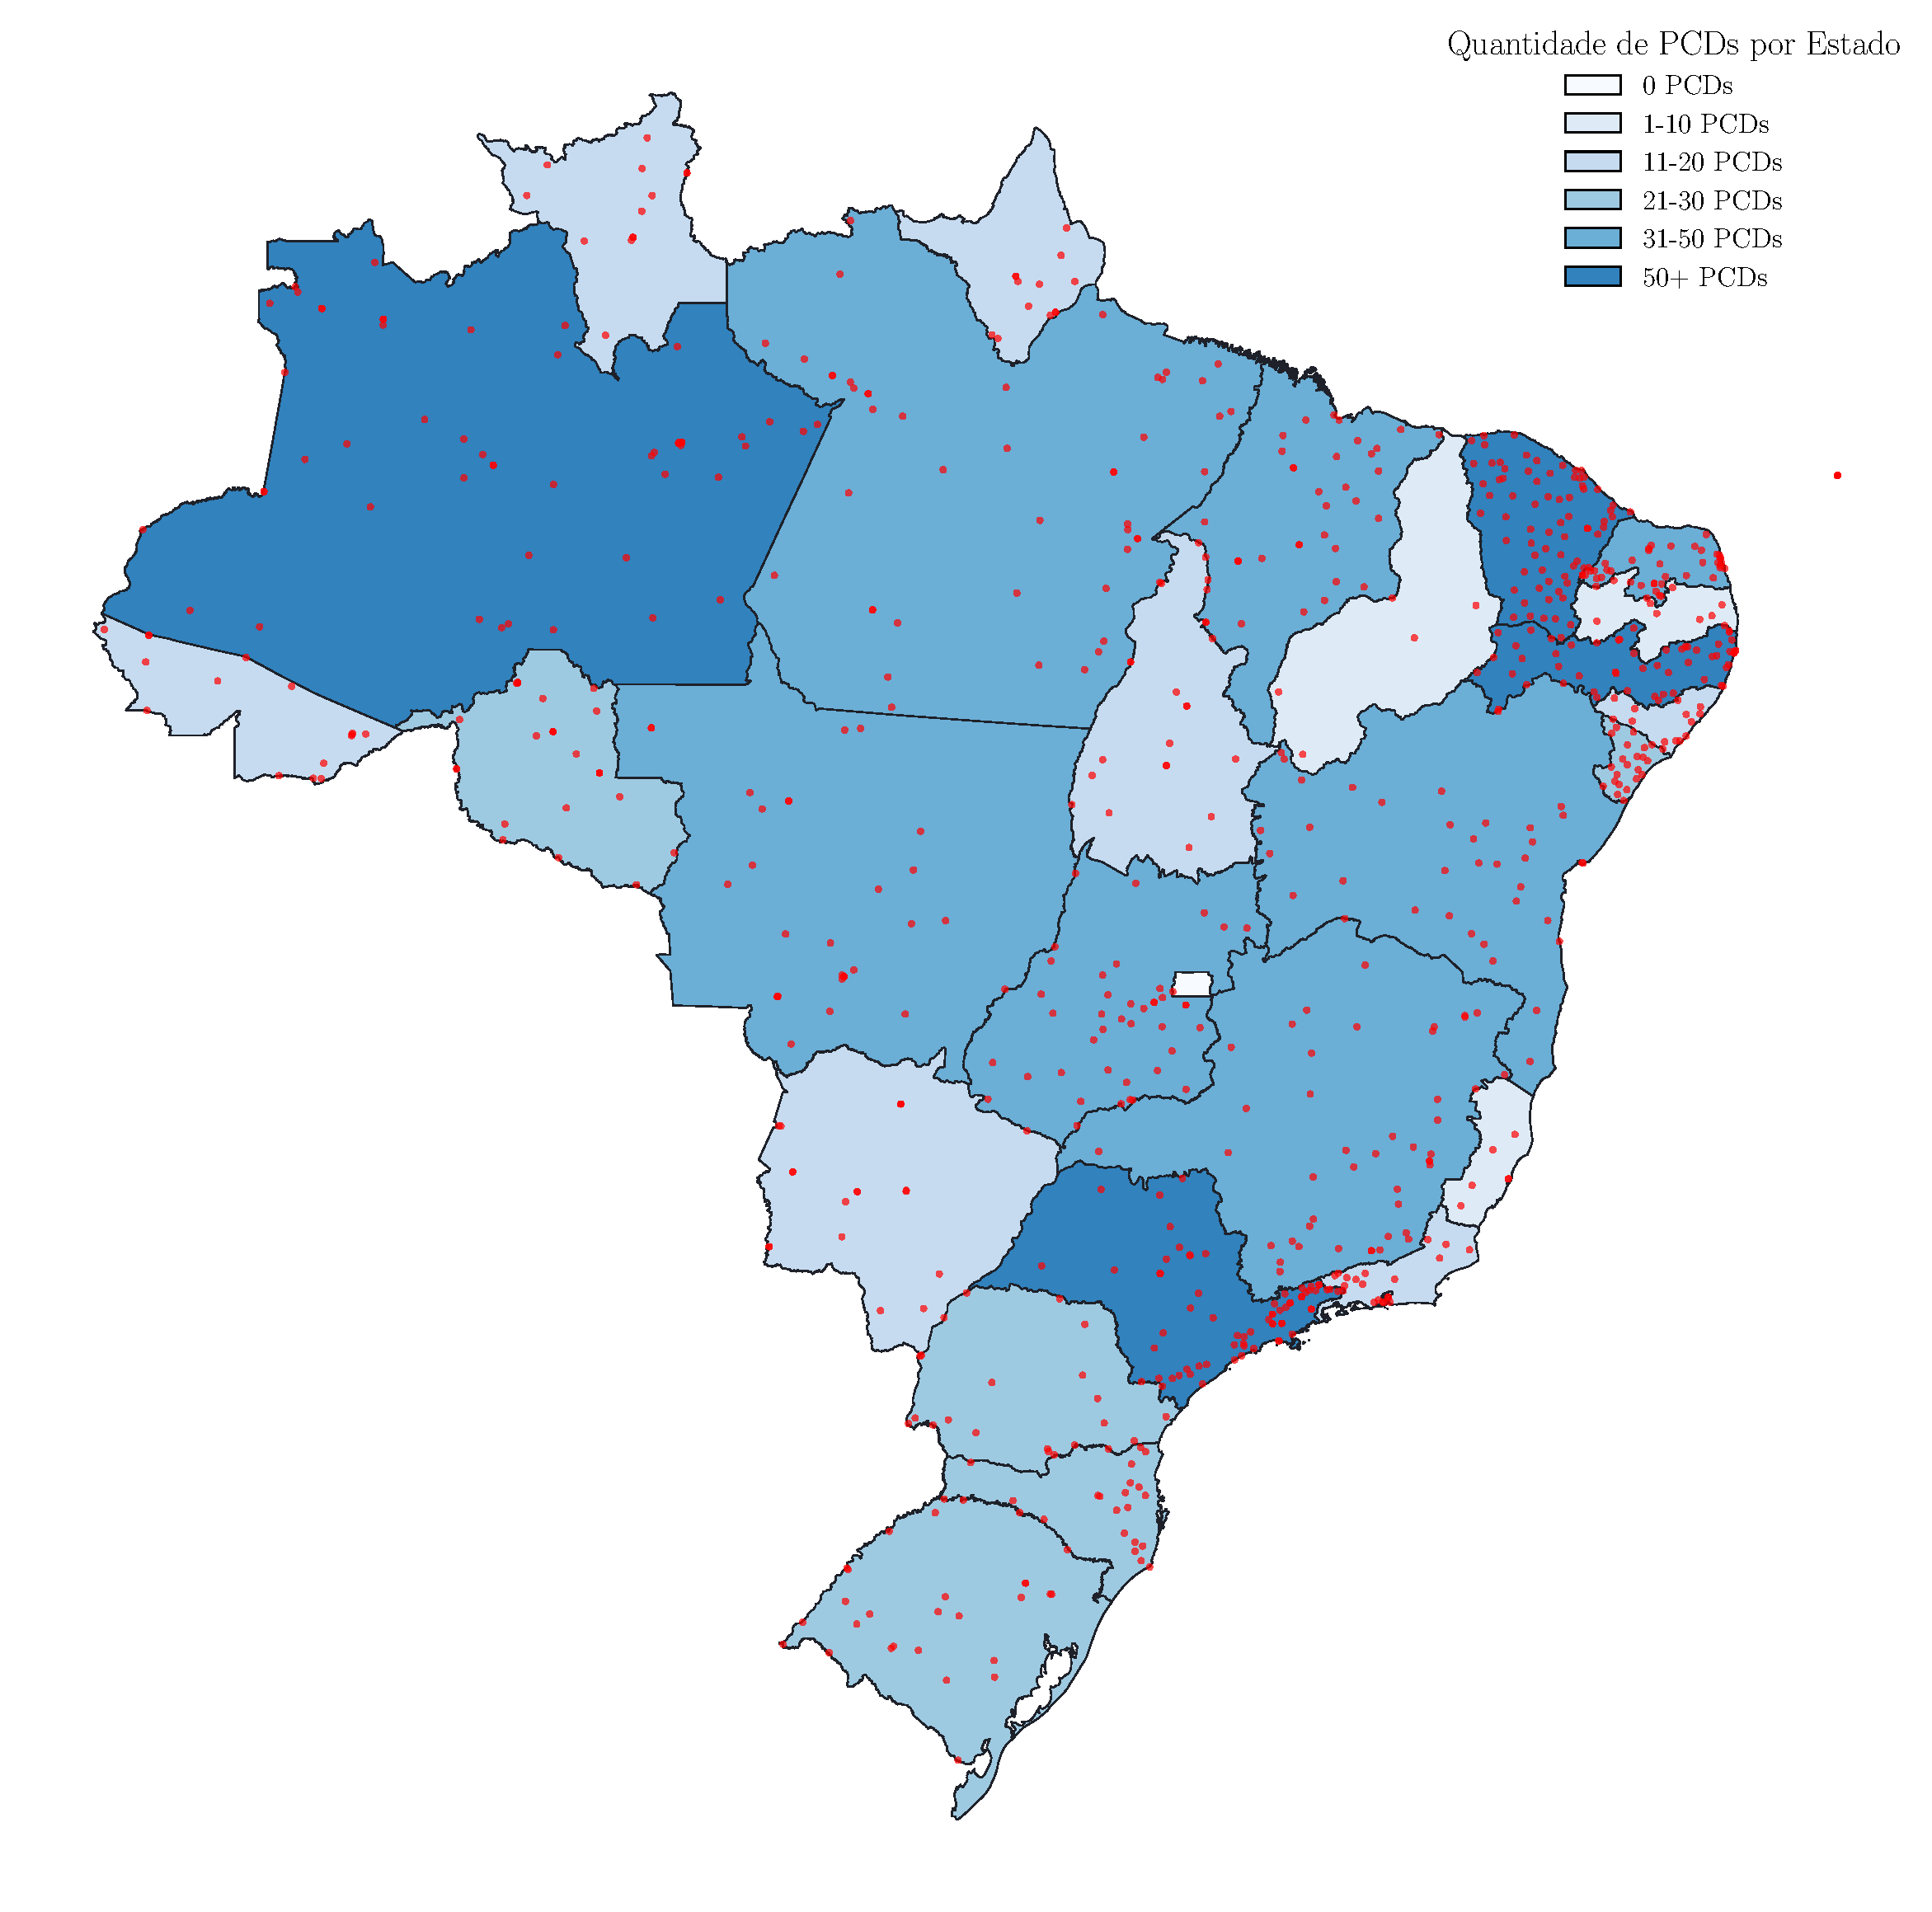
\includegraphics[width=0.95\linewidth]{assets/cap1/geoplot.pdf}
\end{figure}


Grande parte dessas \gls{PCD} é compatível com o padrão \gls{ARGOS-II}, implantado a partir de 1993. Esses dispositivos, entretanto, operam com tecnologias de hardware e software limitadas à época de sua instalação, apresentando restrições quanto à eficiência espectral, robustez contra interferências e capacidade de transmissão de dados. Diante da evolução das demandas de comunicação, da necessidade de aprimorar o desempenho do sistema e da dificuldade na aquisição dos componentes legados para montagem do hardware compativel com \gls{ARGOS-II}, o \gls{ARGOS-III} foi desenvolvido.

O sistema \gls{ARGOS-III} introduziu o uso de transmissores do tipo \gls{PTT-A3} que empregam técnicas digitais mais avançadas, como modulação \gls{QPSK}, codificação convolucional e embaralhamento de dados, visando maior robustez frente a desvanecimentos e erros de rajada. Esses avanços também motivaram o desenvolvimento de novos transmissores e receptores compatíveis com o padrão \gls{PTT-A3} \cite{cnes_services_and_message_formats_ed2_rev2_2006}.

Neste contexto, o presente trabalho tem como objetivo a simulação de um modulador/demodulador compatível com o padrão \gls{PTT-A3}, conforme as especificações do sistema \gls{ARGOS-III}, contribuindo para a formação de massa crítica com domínio técnico sobre os elementos do sistema, a fim de criar melhores condições para que futuros esforços de modernização das \gls{PCD} do \gls{SBCDA} possam ser conduzidos. 


\section{OBJETIVOS}\label{cap:objetivos}

Este trabalho tem como objetivo principal a simulação e análise de um sistema de modulação e demodulação compatível com o padrão \gls{PTT-A3}, utilizado no sistema de satélites \gls{ARGOS-III}. 

\subsection{Objetivo geral}

Simular um sistema de modulação e demodulação compatível com o padrão \gls{PTT-A3} do sistema de satélites \gls{ARGOS-III}.

\subsection{Objetivos específicos}

Para atingir o objetivo geral proposto, este trabalho foi estruturado em uma série de etapas com metas técnicas bem definidas. Os objetivos específicos foram organizados de modo a contemplar a compreensão teórico/pratica do padrão de comunicação \gls{ARGOS-III}. São eles:

\begin{itemize}
   \item Estudar o padrão de comunicação ARGOS; 
   \item Simular a cadeia de transmissão do padrão \gls{PTT-A3}; 
   \item Simular o efeito da adição de ruído;
   \item Simular a detecção de múltiplas portadoras;
   \item Simular a recepção e demodulação do sinal; 
   \item Simular a sincronização de quadros.
   \item Simular a montagem e intepretação do datagrama.
\end{itemize}


\section{ORGANIZAÇÃO DE TEXTO}

O conteúdo deste trabalho está organizado da seguinte forma: O  \autoref{cap:revisao} apresenta a fundamentação teórica necessária para a compreensão do projeto. Já o \autoref{cap:desenvolvimento} descreve o desenvolvimento e as etapas na execução do projeto.